\documentclass[master=cws, masteroption=vs]{kulemt}

% Vul de titel van jouw masterproef hieronder in tussen { en }.
\setup{title={Gametheory and Cybersecurity: a study FlipIt and multiple resources},
%
% Vul hieronder namen in, steeds Voornaam Naam.
% Indien meerdere auteurs, assessoren, assistenten, scheidt hun namen
% met \and .
author={Sophie Marien},
promotor={Prof.\,dr.\,ir.\ Tom Holvoet},
assessor={Ir.\,W. Eetveel\and W. Eetrest},
assistant={Ir.\ Jonathan Merlevede, \ Ir. Kristof Coninx}}
% 
% De volgende \setup mag verwijderd worden als geen fiche gewenst is.
\setup{filingcard,
  translatedtitle={Beste masterproef ooit al geschreven},
  udc=621.3,
  shortabstract={Hier komt een heel bondig abstract van hooguit 500
    woorden. \LaTeX\ commando's mogen hier gebruikt worden. Blanco lijnen
    (of het commando \texttt{\string\pa r}) zijn wel niet toegelaten!
    \endgraf \lipsum[2]}}
% Verwijder de "%" op de volgende lijn als je de kaft wil afdrukken
%\setup{coverpageonly}
% Verwijder de "%" op de volgende lijn als je enkel de eerste pagina's wil
% afdrukken en de rest bv. via Word aanmaken.
%\setup{frontpagesonly}

% Kies de fonts voor de gewone tekst, bv. Latin Modern
\setup{font=lm}

% Hier kun je dan nog andere pakketten laden of eigen definities voorzien
\usepackage{graphicx}
\usepackage{amsmath}
\usepackage{amssymb}
\usepackage{listings}
\usepackage{color}
\usepackage{soul}
\usepackage{tikz}
\usepackage{parskip}
\usepackage{todonotes}
\usepackage{url}
\usepackage{natbib} 
\usepackage{pgf}
\usepackage{tikz}
\usetikzlibrary{arrows,automata}
%\usepackage[latin1]{inputenc}
\definecolor{dkgreen}{rgb}{0,0.6,0}
\definecolor{gray}{rgb}{0.5,0.5,0.5}
\definecolor{mauve}{rgb}{0.58,0,0.82}

\lstset{frame=tb,
  language=Java,
  aboveskip=3mm,
  belowskip=3mm,
  showstringspaces=false,
  columns=flexible,
  basicstyle={\small\ttfamily},
  numbers=none,
  numberstyle=\tiny\color{gray},
  keywordstyle=\color{blue},
  commentstyle=\color{green},
  stringstyle=\color{black},
  breaklines=true,
  breakatwhitespace=true
  tabsize=3
}

%\newcommand{\todo}[1]{{\huge \textcolor{green}{#1}}\\}
%\newcommand{\com}[1]{\textcolor{red}{#1}\\}
%\newcommand{\viscomment}[1]{\textcolor{red}{#1}}
\newcommand{\flip}[1] {\textcolor{black}{#1}}

% Tenslotte wordt hyperref gebruikt voor pdf bestanden.
% Dit mag verwijderd worden voor de af te drukken versie.
\usepackage[pdfusetitle,colorlinks,plainpages=false]{hyperref}

%%%%%%%
% Om wat tekst te genereren wordt hier het lipsum pakket gebruikt.
% Bij een echte masterproef heb je dit natuurlijk nooit nodig!
\IfFileExists{lipsum.sty}%
 {\usepackage{lipsum}\setlipsumdefault{11-13}}%
 {\newcommand{\lipsum}[1][11-13]{\par Hier komt wat tekst: lipsum ##1.\par}}
%%%%%%%

%\includeonly{chap-n}
\begin{document}

\begin{preface}
  I would like to thank everybody who kept me busy the last year,
  especially my promotor and my assistants. I would also like to thank the
  jury for reading the text. My sincere gratitude also goes to my wive and
  the rest of my family.
\end{preface}

\tableofcontents*
\listoftodos
\begin{abstract}
There are many possible ways to attack a company network. Everyday they suffer frrom multiple attakcs and stealthy attacks.
We will make use of a gamemodel FlipIt to find out what the best strategies are for a network manager to defend his network. A worm or a virus will propagate through the network and will cause nodes to be infected. By flipping it the network manager can keep his network clean.
In this thesis I present a work of gametheory merged with cybersecurity. 
  The \texttt{abstract} environment contains a more extensive overview of
  the work. But it should be limited to one page.


\end{abstract}

\begin{abstract*}
  In dit \texttt{abstract} environment wordt een al dan niet uitgebreide
  Nederlandse samenvatting van het werk gegeven.
  Wanneer de tekst voor een Nederlandstalige master in het Engels wordt
  geschreven, wordt hier normaal een uitgebreide samenvatting verwacht,
  bijvoorbeeld een tiental bladzijden. 

  \lipsum[1]
\end{abstract*}

% Een lijst van figuren en tabellen is optioneel
%\listoffigures
%\listoftables
% Bij een beperkt aantal figuren en tabellen gebruik je liever het volgende:
\listoffiguresandtables
% De lijst van symbolen is eveneens optioneel.
% Deze lijst moet wel manueel aangemaakt worden, bv. als volgt:
\chapter{List of Abbreviations and Symbols}
\section*{Abbreviations}
\begin{flushleft}
  \renewcommand{\arraystretch}{1.1}
  \begin{tabularx}{\textwidth}{@{}p{12mm}X@{}}
    LoG   & Laplacian-of-Gaussian \\
    MSE   & Mean Square error \\
    PSNR  & Peak Signal-to-Noise ratio \\
  \end{tabularx}
\end{flushleft}
%\section*{Symbols}
%\begin{flushleft}
%  \renewcommand{\arraystretch}{1.1}
%  \begin{tabularx}{\textwidth}{@{}p{12mm}X@{}}
%    42    & ``The Answer to the Ultimate Question of Life, the Universe,
%            and Everything'' according to \cite{h2g2} \\
%    $c$   & Speed of light \\
%    $E$   & Energy \\
%    $m$   & Mass \\
%    $\pi$ & The number pi \\
%  \end{tabularx}
%\end{flushleft}

% Nu begint de eigenlijke tekst
\mainmatter

\chapter{Introduction}
\label{cha:intro}
The first contains a general introduction to the work. The goals are
defined and the modus operandi is explained.
\todo{bib referenties in orde brengen}
\section{Introduction}

Security is an important asset in Computer Science. Defending a network of a company is not an easy job. To prevent intruders it can make use of firewalls, routers, IDS systems, virus scans, and other defence mechanisms. Unfortunately technology is growing fast and attacks are getting more sophisticated and the causes of these attacks can be very different. \todo{iets tussen nog} Companies are often the victim of targeted attacks. In a security report of 2014, \todo{verwijzing naar report}, states that 80\% of the companies are the victims of targeted attacks. Many companies don't see themselves as a target, but sometimes they might be collateral, the target on the way to the real target. This means that everybody can be a target. 
Corporate networks should continuously defend themselves against outside invaders such as viruses and worms. By doing so the network administrator can keep the network as malware-free as possible. If there is  an intruder managed to penetrate the network then the network manager this intruder trying to get out as quickly as possible. This is not always easy. Especially when the intruders secretly sneak and then spread rapidly.
In this paper we will work further on the work made by Marten van Dijk, Ari Juels, Alina Oprea and Ronals L. Rivest \todo{verwijzing naar FlipIT} who wrote a report on the Game FlipIt. FlipIt is a the game of '' Stealthy Takeovers''. It models a game by means of two players, the attacker and the defender. Both can gain control over a single shared resource by flipping it. The most important property of the game is that the flipping happens stealthy. This means that the players have no clue about when the other player moves. The goal of the game is to maximise the time the player controls the resource minus the average cost of the flipping. 

\subsection{Motivation of the game}
%waarom FlipIt gebruiken en niet iets anders.
\subsection{Contributions and results}
\subsection{Conclusions}
The "I love you" virus is an example of a virus that spreads quickly. This virus propagates via mail systems. If someone opens an email with "I love you" virus in annex this virus spreads itself by sending a mail itself to everyone in your contact list. So the virus can multiply rapidly and eventually a business network shut down by the heavy traffic. In this example, there is a need human interaction to spread the virus to do. If no one opens the virus can not spread the mail.
Unfortunately, there are viruses that can spread without human interaction. These viruses are referred to as worms. A worm is also a computer program that replicates itself to spread to other computers so. Via a computer network, copies of the worm forwarded without an intermediary is used for. The worm will use vulnerabilities to infect other computers.
Most worms are designed to spread out and just try not to make any changes to the systems that they pass. These worms can still inflict damage by increased network traffic they generate. Worms that contain Harm damage a program to install a backdoor or a rootkit on the infected computers. Backdoors and rootkits ensure that future use can be made of the infected computers.
The Stuxnetworm is a very famous worm. Initially this worm spread via infected USB sticks and from then it could spread through the Internet to other computers. The purpose of the Stuxnetworm was broken to run the centrifuges in nuclear reactors. Many reactors have been infected. From the standpoint of the defender, it is very important to respond as quickly as possible so that the worm can not spread quickly.

\section{introduction number 2}

(We live in an era) In this era where digitalization becomes prominent in every aspect of our lives, where technology is growing fast and where business are always under attack, security becomes an issue of increasing complexity. Since 2009, the number of reported security attacks has increased 66\%, year over year. \todo{security report van pwc}. These numbers only represent the attacks that are detected. In 2014 117,339 attacks where coming in daily. Many of those attacks have a different cause. Some of them can be benign, others can be harmful. Many companies are unaware of all the attacks. Some of them think that they are not a target, but they might be a target on the way to a real target. Recently there where some high profiled targeted attacks which have been revealed. (Belgacom). 
Targeted attacks are ...
The \textit{Kill Chain} is a concept by Lockheed Martin Corporation, explained in the whitepaper \todo{withepaper toevoegen}. It explains the different phases of a typical attack from the view of an attacker. It also outlines the typical attacker activities on the right. This model is very useful to define the different moments of the life cycle of an attack and when a company should act to defend itself. In this paper we would like to prevent the viruses of spreading into the network system of a company. This means that we have to act in phase Installation, Command and Control and Action on Objectives of the kill chain. 

 
  Security is an important asset in Computer Science. Defending a network of a company is not an easy job. Malicious people will try to  To prevent intruders it can make use of firewalls, routers, IDS systems, virus scans, and other defence mechanisms. Unfortunately technology is growing fast and attacks are getting more sophisticated and the causes of these attacks can be very different. \todo{iets tussen nog} Companies are often the victim of targeted attacks. In a security report of 2014, \todo{verwijzing naar report}, states that 80\% of the companies are the victims of targeted attacks. Many companies don't see themselves as a target, but sometimes they might be collateral, the target on the way to the real target. This means that everybody can be a target. 
Corporate networks should continuously defend themselves against outside invaders and targeted attacks. Researchers have already investigated the situations through the FlipIt game in which a system is continuously compromised by an attacker through targeted attacks. 
FlipIt is a the game of '' Stealthy Takeovers''. It models a game by means of two players, the attacker and the defender. Both can gain control over a single shared resource by flipping it. The most important property of the game is that the flipping happens stealthy. This means that the players have no clue about when the other player moves and has control over the shared resource. The goal of the game is to maximise the time the player controls the resource minus the average cost of the number of flipping.
In this paper we model a company network through multiple shared resources and a flip from the attacker that drops a virus that will spread itself autonomously. We show that ...

%\begin{minipage}{0.5\textwidth}
%\includegraphics{Images/killchain.jpg}
%\end{minipage} \hfill
%\begin{minipage}{0.45\textwidth}
%\begin{itemize}
%\item *Rectangle
%\item *Color: blue
%\end{itemize}
%\end{minipage}

%http://www.pwc.com/gx/en/consulting-services/information-security-survey/index.jhtml
%%% Local Variables: 
%%% mode: latex
%%% TeX-master: "thesis"
%%% End: 


\chapter{The FlipIt game}
\label{cha:2}


\section{Extensions on FlipIt}


There a various possible ways to extend \flip{FlipIt}. For instance Laszka et al. extended the basic \flip{FlipIt} game to multiple resources. The incentive is that for compromising a system in a real case it needs more than just taking over one resource. An example is gaining access to a system and breaking the password. The model is called FlipThem \cite{FlipThem}. Two ways of flipping the resources are used: the AND and the OR control model. In the AND model the attacker only controls the system if he controls all the resources of the system, whereas in the OR model the attacker only needs to compromise one resource to be in control of the entire system. The difference with FlipThem and this paper is that we introduce a Graph Model in the beginning.\\
Another extension on FlipIt is done by Pham [\todo{citatie needed voor Are We Compromised?}]. Beside the action Flip their is another action Test. The basic idea is to test with an extra action if the resource has been compromised or not. This action involves also an extra cost. This model is useful if somebody wants to know for example if his password has been compromised or wants to assess the periodic security of a system.  In \citep{MitigationCovert} \cite{MitigationNonTargeted} Laszka et al. they also consider non targeted attacks by non-strategic players and \todo{verder aanvullen}. 








In this section, we introduce the game \flip{FlipIt} \cite{FlipIt}. \flip{FlipIt} is a game introduced by .. .. and Rivest. First we explain the framework of FlipIt and after that the formulas and assumptions that we will make for the game for during the whole paper.  

\section{The First Topic of this Chapter}
\flip{FlipIt} is a two-players game with a shared (single) resource that the players want to control as long as possible. The shared resource can be a password, a network or a secret key depending on the setting being modelled. In the rest of the paper we will call the players the Attacker and the Defender. To get the control over the resource, players can flip the resource at any given time. Each move will imply a certain cost. The unique feature of \flip{FlipIt} is that the move will happen in a stealthy way, meaning that the other player has no clue that the other player has flipped the resource. For instance, the defender will not find out if the resource has already been compromised by the attacker, but he can only potentially know it after he flips the resource himself. The goal of the player is to maximize the time that he or she has control over the resource while minimizing total cost of the moves. Players won't move to frequently. A move can also result in a "wasted move", called a flop. It may happen that the resource was already under control by the defender. If the defender moves when he or she has already control over the resource, he or she would have wasted move since it does not result in a change of ownership. 
 
Because the players move in a stealthy way, there are different types of feedback that a player can get while moving:
\begin{itemize}
\item Non-adaptive (NA): The player does not receive any feedback while flipping.
\item Last move (LM): The player finds out the exact time the opponent played the last time.
\item Full History (FH): The player finds out the complete history of the opponents move.
\end{itemize}
The game can be extended by the amount of information that a player receives. It can also be possible for a player to get information at the start of the game. Both interesting cases are:
\begin{itemize}
\item Rate-of-play (RP: The player finds out the exact rate of play of the opponent.
\item Knowledge-of-strategy (KS): The player finds out the complete information of the strategy that the opponent is playing.
\end{itemize}

In our assumption the strategy of both players will be non-adaptive. None of the players has information of the strategy of the opponent. 



\section{Figures}
\begin{figure}[hbtp]
\centering
\includegraphics[scale=0.25]{Images/FlipItDefault.jpg}
\caption{The FlipIt game where both players are playing periodically}
\label{fig:FLipItDefault}
\end{figure}
\todo{verwijzen naar de figuur \ref{fig:FLipItDefault}}

\subsection{Strategies}
 
 In this subsection we go through the strategies used in FlipIt and the most important results. 
 \begin{table}
 \centering
 \begin{tabular}{ l | c  }
  \textbf{Categories} & \textbf{Classes of Strategies} \\
  \hline Non-adaptive (NA) & Exponential \\
  & Periodic \\
  & Renewal \\
  & General non-adaptive \\
  \hline Adaptive (AD) & Last move (LM) \\
  & Full History (FH) \\  
\end{tabular}
 \caption{Classes of strategies in FlipIt}
 \label{table:Strategies}
 \end{table}

There are two different kinds of strategies, the \textit{non-adaptive strategies} and the \textit{renewal strategies}. If there is no need for feedback for both of the players, we say that we have a non-adaptive strategy. Because the player does not receive any feedback during the game it will play in the same manner against every opponent. They are not dependent on the opponents movements. This means that they can already generate the time sequence for all the moves in advance.  But they can depend on some randomness because the non-adaptive strategies can be randomised. 
In this paper we will focus in the beginning on the non-adaptive strategies. Reasons behind this that a player (defender or attacker) rarely knows what the strategies are of his opponent. [If the attacker wants to move stealthily, it might have limited attack options FLIPTHEM]. \todo{nog redenen zoeken}\\
A renewal strategy is a non-adaptive strategy where the time intervals between two consecutive moves are generated by a renewal process. \\

 \begin{description}
 \item Periodic
 \item Non-Arithmetic Renewal
 \item Exponential
 \end{description}

\section{Formal definition Game}

In this section we provide the formal definition of the game and the notation that we will use throughout the paper.

\begin{description}
\item \textit{Players}  There are two players in the game, one is the defender and the other one is the attacker. They are respectively identified by 0 and 1.
\item \textit{Time}  The game starts at $t=0$ and continuous indefinitely as $t \rightarrow \infty$. The game is a continuous game.
\item \textit{Game State} There is also a time-dependent variable that represents the state of the game. $C=C(t)$ is either 0 if the Game is under control by the defender and 1 if the Game is under control by the attacker. We can also define the state of each resource by $C^{A}$ and $C^{D}$. If $C^{A} = 1$ then this means that the attacker has control over the resource, and 0 otherwise. For $C^{D}$ it is visa versa, $C^{D} = 1 - C^{A}$.
\item \textit{Graph} We represent the company network as a Graph $G = < V,E>$. G is an ordered pair where V denotes the set of resources or nodes in the network and E denotes the set of connections or links, which are a two-element subset of V. We use the notations resources and nodes interleaving in this paper.\\
We have N resources in the network. $N \in $  \todo{aanvullen}. This means we can denote the resources by:
\begin{center}
$V \in {V_{0}, V_{1}, V_{2}, ... , V_{N} }$
\end{center}
The set E of connections indicates if there is a link between two resources. We see the links as bidirectional so the total graph is undirected. If there is a link between resource $V_{n}$ and $V_{n+1}$ then there is also a link between $V_{n+1}$ and $V_{n}$. 

\item \textit{Moves} Both players can make a move in the game. Moves done in a finite numbers of time in any finite time interval. Both players can play at any time they want, they can also play at the same time. If this happens the one that has control over the resource will keep having control over the resource.
This makes the game fully symmetric \todo{beter uitleggen}. The sequence of move times are denoted by the following infinite sequence:
\begin{center}
$t=t_{1},t_{2},t_{3},..$
\end{center}
Two move times can be the same because we allow players to move at the same time.
We can also denote the infinite sequence of times when player \textit{i}  moves. We write this as :
\begin{center}
$t=t_{i,1},t_{i,2},t_{i,3},..$ with \textit{i} $ \in $ $\lbrace 0,1 \rbrace$
\end{center}
The sequences $t_{1}$ and $t_{0}$ are disjoint subsets of the sequent t. 
We can also denote who made the \textit{k}th move by defining a sequence \textit{p} that denotes the sequence of who played:
\begin{center}
$p=p_{1},p_{2},p_{3}, .. $ with $p_{k}$ $\in$ $\lbrace 0,1 \rbrace$
\end{center}

\item \textit{Number of moves}  $n_{i}(t$ denotes the number of moves made by player \textit{i} up to and including time t. This means that 
\begin{center}
$n(t)=n_{1}(t) + n_{0}(t)$
\end{center}
is the sum of the number of moves made by the defender and the attacker up to and including time t. 

\item \textit{Average move rate} We denote $\alpha_{i}(t)$ as the average move rate by player i:
\begin{center}
$\alpha_{i}(t) = n_{i}(t)/t$ with $t > 0$ and \textit{i} $ \in $ $\lbrace 0,1 \rbrace$
\end{center}

\item \textit{Period} We can also define the period in terms of the average move rate:
\begin{center}
$\delta_{i}=1/\alpha_{i}$
\end{center}

\item \textit{Cost} The cost is an important property of the game. In FlipIt for every player the cost of a move is denoted by $k_{i}$. These costs can be very different for every player. In this game we denote the players flipping cost for resource $V_{N}$ by $c_{i}^{V_{N}}$. \\
For the defender the cost will be either the cost of flipping every resource or the cost of flipping a subgroup of the resources.\\
For the attacker the cost will be the cost of dropping a virus on a node. The spreading of the virus will not imply an extra cost. 

\item \textit{Utility} In FlipIt the Gain definition is the utility function. The Gain denotes the total time a player i has gained control over a resource. \todo{nu gain van een resource, moet voor verschillende resources zijn}
The Gain $G_{i}$ denotes players i total gain of a game, wich is the total time the player has gained control over a subset of resources thus controlling the game. If we sum up the total Gain of the attacker and the defender we end up with the time:
\begin{center}
$G_{1}(t) + G_{0}(t) = t$
\end{center}
\item \textit{Average gain rate} The average gain rate for player i is defined as
\begin{center}
$\gamma_{i}(t)= G_{i}(t)/t$
\end{center}

\subsection{Our Game parameters}
\begin{description}
\item \textit{Graph Matrix} We represent the graph of the network through a matrix $ A = |V| \times |V|$. The (i,j)-entry of the matrix A will have a 1 if there is a connection between node $V_{i}$ and node $V_{j}$. If we are working with an undirected graph the matrix will be symmetric. 
\item \textit{Attack Vector} We denote $X = 1 \times |V|$ as the attack vector.  
\item \textit{Reset vector} The reset vector will make sure that the right entries in the matrix become zero.
\item \textit{Cummulative Matrix} 
\item \textit{State Matrix} The State matrix $T(t) = |V| \times |V| $ will keep at every time t the state of the game.
\end{description}

\end{description}


\section{Conclusion}
The final section of the chapter gives an overview of the important results
of this chapter. This implies that the introductory chapter and the
concluding chapter don't need a conclusion.



%%% Local Variables: 
%%% mode: latex
%%% TeX-master: "thesis"
%%% End: 

\chapter{Intoduction to GameTheory}
\label{cha:1}
%\documentclass[10pt]{article}
%\begin{document}

%%%%%%%%%%%%%%%%%%%%%%%%%%%%%%%%%%%%%%%%%%%%%%%%%%%%%%%%%%
%%%%%			Introduction Chapter 1				%%%%%%
%%%%%												%%%%%%
%%%%%												%%%%%%
%%%%%%%%%%%%%%%%%%%%%%%%%%%%%%%%%%%%%%%%%%%%%%%%%%%%%%%%%%

Gametheory is a mathematical study to analyse interactions between independent and self-interested agents. To get an understanding of the most important concepts of game theory, a short introduction based on the work of 
\citep{leyton2008essentials} and \todo{Coursera} is given in section 2.1 [] \todo{ref}. For a more detailed and full introduction to game theory, the reader is referred to 
\todo{leyton2008essentials}.  In section 2.2 [] \todo{ref} an overview of the FlipIt game is given with the definitions and concepts that will be used throughout the paper.
The last section [] \todo{ref} will cover the extensions and additions already made on FlipIt.

%------------------------------------------------%
%            Intro Game Theory 					 %
%------------------------------------------------%
\section{A brief introduction in Game Theory}
\label{Cha:1:Intro.Game.Theory}



%begin over dat gametheorie handig is in de economie

Game theory studies the interaction between independent and self-interested agents. It is a mathematical way of modelling the interactions between two or more agents where the outcomes depend on what everybody does and how it should be structured to lead to good outcomes. For this reason it can be very useful in economics and also in other branches as politics, biology, computer science, philosophy and a variety of other disciplines.  \\
%Every agent has different levels of happiness for the different outcomes.
%self interested meaning

One of the assumptions underlying game theory is that the players of the game, the agents, are independent and self-interested. This does not necessarily mean that they want to harm other agents or that they only care about themselves. 
%utility function meaning 
Instead it means that each agent has preferences about the states of the world he likes. These preferences are mapped to natural numbers and are called the utility function. The numbers are interpreted as a mathematical measure to tell you how much an agent likes or dislikes the states of the world. \\
It also explains the impact of uncertainty. When an agent is uncertain about a distribution of outcomes, his utility will describe the expected value of the utility function with respect to the probability of the distribution of the outcomes. For example: with 0.7 probability it will be 7 degrees outside and 0.3 probability it will be 10 degrees. The agent can have a different opinion about that distribution versus another distribution. (\todo{uitleggen aan de hand van een voorbeeld}).\\
\todo{players rationeel en max outcomes}
%Cooperative and non cooperative games
In a Decision Game Theoretic Approach an agent will try to act in such a way to maximise his expected or average utility function. It becomes more complicated when two or more agents want to maximise their utility and whose actions can affect each other utilities. This kind of games are referred to as non-cooperative game theory, where the basic modelling unit is the group of agents. The individualistic approach, where the basic modelling is only one agent, is referred as cooperative game theory. 

%There are two standard representations for games. The first one is the Normal Form. The second one is the Extensive Form.

In the following list a couple of terms that will be used throughout the paper.
\begin{description}
\item \textit{Players}: Players are referred as the ones who are the decision makers. It can be a person, a company or an animal.  (they will act rational )
\item \textit{Actions}: Every player has actions that he or he can do. 
\item \textit{Strategies}: A strategy is the combination of different actions. A pure strategy is only one action.
\item \textit{Utility function}: The utility function is the mapping of the level of happiness of an agent about the state of the world to natural numbers.

\end{description}

A game in game theory consists of multiple agents and every agent has a set of actions that he can play. 

\todo{strategien en acties definieren}

%Nash equilibrium

%John Nash speelde ook een grote rol in de geschiedenis van de speltheorie. Hij is een van de wiskundigen geweest die speltheorie geformaliseerd heeft. Het Nash evenwicht werd naar hem vernoemd. Een Nash evenwicht wordt gezien als een evenwicht tussen beide spelers zodat ze allebei de beste tactiek kiezen en niet meer veranderen als de andere van tactiek veranderen. John Nash breide de theorie over het Nash evenwicht in een paper nog uit met gemengde strategieën. In 1994 kreeg John Nash samen met twee andere wiskundigen gespecialiseerd op het vlak van speltheorie de Nobelprijs voor de economie op basis van hun prestaties in de niet-coöperatieve speltheorie. . Over John Nash is een prachtige film 
\subsection{Best response and Nash Equilibrium}
One of the solution concepts in Game Theory for non-cooperative games is a Nash Equilibrium that we will use in this paper. A Nash Equilibrium is a subset of outcomes that can be interesting to analyse a game. For a Nash Equilibrium each player has a consist list of actions and each player's action maximizes his or her payoff given the actions of the other players. Nobody has the incentive to change his or her action if an equilibrium profile is played. In general we can say that a Nash Equilibrium is a stable strategy profile: each player is considered to know the equilibrium strategies of the other players and no player would want to change his own strategy if he knows the strategies of the other players. 

Formal defenition of a Nash Equilibrium:
A strategy profile $s = (s1, . . . , sn)$ is a Nash equilibrium
if, for all agents $i$, $si$ is a best response to $s-i$ .
''Intuitively, a Nash equilibrium is a stable strategy profile: no agent would want to change
his strategy if he knew what strategies the other agents were following.
Wecan divide Nash equilibria into two categories, strict and weak, depending on whether
or not every agent's strategy constitutes a unique best response to the other agents' strategies.''

\todo{Nash beter uitleggen nog met best response erbij}


POSTCONDITION: Uitgelegd: Strategien, acties, strategien, spelers, rationeel, Nash, best response
%In game theory, the Nash equilibrium is a solution concept of a non-cooperative game involving two or more players, in which each player is assumed to know the equilibrium strategies of the other players, and no player has anything to gain by changing only their own strategy.[1] If each player has chosen a strategy and no player can benefit by changing strategies while the other players keep theirs unchanged, then the current set of strategy choices and the corresponding payoffs constitutes a Nash equilibrium. The reality of the Nash equilibrium of a game can be tested using experimental economics method.

%In de speltheorie, een deelgebied van de wiskunde, is een Nash-evenwicht een oplossingsconcept voor een niet-coooperatief spel, waar twee of meer spelers aan meedoen. In een Nash-evenwicht wordt elke speler geacht de evenwichtsstrategieeen van de andere spelers te kennen en heeft geen van de spelers er voordeel bij om zijn of haar strategie eenzijdig te wijzigen. Als elke speler een strategie heeft gekozen en geen enkele speler kan profiteren door zijn strategie te veranderen, terwijl de andere spelers dat ook niet doen, dan vormt de huidige verzameling van strategiekeuzes plus de bijbehorende uitbetalingen een Nash-evenwicht. 

%Een Nash-evenwicht gaat uit van een spel, waarin iedere speler een strategie heeft. Die strategie geeft precies aan wat een speler in de verschillende fases van een spel doet. Een strategie kan zowel een pure strategie als een gemengde strategie zijn. De verzameling van strategieeen van alle spelers die meedoen aan een bepaald spel noemt men een strategieprofiel. In de speltheorie is een Nash-evenwicht een strategieprofiel waarbij het voor geen enkele speler voordelig is daarvan af te wijken, als de andere spelers dat ook niet doen.

%Het Nash-evenwichtsconcept is een begrip dat vooral toepassing vindt in de economie.


\section{The FlipIt game}
In this section, we introduce the ''stealthy takeover '' game \flip{FlipIt} \cite{FlipIt}. \flip{FlipIt} is a game introduced by van Dijk et al. First we explain the framework of FlipIt and introduce the most important formules that will be used throughout the paper. To understand how to model a FlipIt game with virus propagation it is important to get familiar with the concepts of the normal FlipIt game and it's notations.  \\

\flip{FlipIt} is a two-players game with a shared (single) resource that the players want to control as long as possible. The shared resource can be a password, a network or a secret key depending on the setting being modelled. In the rest of the paper we name the two players the attacker, denoted by the subscript \textit{A} and the defender, denoted by subscript \textit{D}. 

The game begins at $t=0$ and continuous indefinitely ($t \rightarrow \infty $). The time in the game can be viewed as being continuous, but a discrete time can also be viewed. To get control over the resource, the players \textit{i} can flip the resource at any given time. A flip will be regarded as a move from a player \textit{i}. Each move will imply a certain cost $k_{i}$ and the cost can vary for each player. Both players will try to minimize their cost. By adding a cost, it will prevent players to move to frequently. \\

The unique feature of \flip{FlipIt} is that every move will happen in a stealthy way, meaning that the player has no clue that (his adversary) the other player has flipped the resource. For instance, the defender will not find out if the resource has already been compromised by the attacker, but he can only potentially know it after he flips the resource himself. The goal of the player is to maximize the time that he or she has control over the resource while minimizing total cost of the moves. A move can also result in a "wasted move", called a flop. It may happen that the resource was already under control by the defender. If the defender moves when he or she has already control over the resource, he or she would have wasted a move since it does not result in a change of ownership and a cost is involved. \\


\begin{figure}[hbtp]
\centering
\includegraphics[scale=0.8]{Images/DefFlipit}
\caption{A representation of a FlipIt game where both players are playing periodically and discrete. Every move or flip is indicated by a blue or orange circle. The attacker is the orange colour and plays with a period of $\delta_{A}=4$. The defender is the blue colour and plays with a period of $\delta_{D}=3$.The blue and orange rectangles represent the amount of time one of the players is in control of the resource.}
\label{fig:FLipItDefault}
\end{figure}
\todo{verwijzen naar de figuur \ref{fig:FLipItDefault}}


The state of the resource is denoted as a time independent variable $C=C_{i}(t)$. 
$C_{D}(t)$ is either 1 if the game is under control by the defender and 0 if the game is under control by the attacker. For $C^{A}(t)$ it is visa versa, $C^{A}(t)= 1 - C^{D}(t)$.\\ \\
The game starts with defender being in control of the game, $C_{D}(0)= 1$. 

The players receive a benefit equal to the time of units that they were in possession of the resource minus the cost of making their moves. The cost of a player \textit{i} is denoted by $k_{i}$. 
The total gain of player \textit{i} is equal to the total amount of time that a player \textit{i} has owned the resource from the beginning of the game up to time \textit{t}. It is expressed as follows:
\begin{equation}\label{first}
G_{i}(t) = \int_0^1 \! C_{i}(x) dx.
\end{equation}
If we add up the gain of the defender and the gain of the attacker it should sum up to t:
\begin{equation}\label{first}
G_{D}(t) + G_{A}(t) = t
\end{equation}
The average gain of player \textit{i} is defined as:
\begin{equation}\label{first}
\gamma_{i}(t) = G_{i}(t)/t.
\end{equation}
And thus for all $t > 0$ :
\begin{equation}\label{first}
\gamma_{D}(t) + \gamma_{A}(t) = 1
\end{equation}
Let $\beta_{i}(t)$ denote player's \textit{i} average benefit upto time \textit{t}:
\begin{equation}\label{first}
\beta_{i}(t) = \gamma_{i}(t) - k_{i}\alpha_{i}.
\end{equation}
This is equal to the fraction of time the resource has been owned by player \textit{i}, minus the cost of making the moves. ~$ \alpha_{i}$ defines the average move rate by player \textit{i} up to time \textit{t}.
In a give game, the asymptotic benefit rate or simply benefit will be defined as the lim inf of the average benefit because time t will increase to infinity and the average benefit may not have limiting values.
\[ \beta_{i}(t)  = \lim_{t \to \infty} inf \beta_{i}(t)  \]
\\


\subsubsection{strategies}
Because the players move in a stealthy way, there are different types of feedback that a player can get while moving. These types of feedback can be divided into two groups of strategies. The non-adaptive strategies and the adaptive strategies. These are described in table \ref{table:Strategies}. \\

If there is no need for feedback for both of the players, we say that we have a non-adaptive strategy. Because the player does not receive any feedback during the game it will play in the same manner against every opponent. They are not dependent on the opponents movements. This means that they can already generate the time sequence for all the moves in advance.  But they can depend on some randomness because the non-adaptive strategies can be randomised. 
In this paper we will focus in the beginning on the non-adaptive strategies. Reasons behind this is that a player (defender or attacker) rarely knows what the strategies are of his opponent. An interesting subclass of the non-adaptive strategies is one where the time intervals between two consecutive moves are generated by a renewal process. Example of such a renewal strategy is the periodic strategy where the time between two consecutive moves of the players are a fixed interval. An exponential strategy is a renewal strategy in which the interval between two consecutive moves is exponentially distributed.  \\

-- Ik kan dit ook pas uitleggen als ik mijn FlipIt spel met virus propagatie uit de doeken doe -- \\
We elaborate more about the periodic strategy because we will use this one to model our first extension. For more details about the other strategies of FlipIt we refer the reader to [the paper of FlipIt].

\textit{periodic strategy}: A Periodic strategy is a non-adaptive renewal strategy where the time intervals between consecutive moves are a fixed period, denoted by $\delta$. Moreover it has a random phase, that is chosen uniformly and random in the interval $[0,\delta]$ for the first move. The average rate of play is denoted by $\alpha = \dfrac{1}{\delta}$. \\

In the category Adaptive strategy there are two sub classes of strategies. The first one is the Last move (LM). In this class whenever a player flips it will find out the exact time that the opponent played the last time. In the second class the Full History (FH), whenever a player flips it will find out the whole history of the opponents move. If the opponent player plays with a renewal strategy the sub classes FH and LM collapse. \\
 I%n this subsection we elaborate about the strategy of FlipIt . 
%A renewal strategy is a non-adaptive strategy \\


 
The game can be extended by the amount of information that a player receives. It can also be possible for a player to get information at the start of the game. Both interesting cases are:
\begin{itemize}
\item Rate-of-play (RP): The player finds out the exact rate of play of the opponent.
\item Knowledge-of-strategy (KS): The player finds out the complete information of the strategy that the opponent is playing.
\end{itemize}




 

 \begin{table}
 \centering
 \begin{tabular}{ l | c  }
  \textbf{Categories} & \textbf{Classes of Strategies} \\
  \hline Non-adaptive (NA) & Exponential \\
  & Periodic \\
  & Renewal \\
  & General non-adaptive \\
  \hline Adaptive (AD) & Last move (LM) \\
  & Full History (FH) \\  
\end{tabular}
 \caption{Hierarchy of Classes of strategies in FlipIt}
 \label{table:Strategies}
 \end{table}




\subsubsection{Imporant results}

\begin{itemize}
\item periodische spellen domineren de andere renewal strategies
\item periodische strategien wel slecht tegen attacker die laatste move weet
\item als de defender snel speelt dan forceert die de attacker om niet meer mee te spelen
\item iedereen die feedback krijgt heeft meer benefit dan zonder die feedback
\end{itemize}
 
\section{Extensions on FlipIt}

In this section we discuss the extensions that can be made on the FlipIt game. \\


There a various possible ways to extend \flip{FlipIt}. 
Laszka et al. made a lot of additions and extensions on the original game of FlipIt. For instance Laszka et al. extended the basic \flip{FlipIt} game to multiple resources. The incentive is that for compromising a system in a real case it needs more than just taking over just one resource. An example is that one resource can be gaining access to a system and breaking the password of the system is another resource. The model is called FlipThem \cite{FlipThem}. They use two ways to flip the multiple resources: the AND and the OR control model. In the AND model the attacker only controls the system if he controls all the resources of the system, whereas in the OR model the attacker only needs to compromise one resource to be in control of the entire system. \\
%The difference with FlipThem and this paper is that we introduce a Graph Model in the beginning.\\
Another addition of Laszka et al. to the game of FlipIt [mitigating covert compromises] is extending the game to also consider non-targeted attacks by non-strategic players. In this game the defender tries to maintain control over the resource that is subjected to both targeted and non-targeted attacks. Non-targeted attacks can include phishing, while targeted attacks may include threats delivered through zero day attack vulnerabilities. \\
One of the last important addition from Laszka et al. [Mitigation of Targeted and] is to consider a game where the moves made by the attacker are still covert but the moves made by the defender are known to the attacker. This means that the attacker can base his attacks on the defender's moves. Both the targeted and non-targeted attacks don't succeed immediately. For the targeted attack the time till it succeeds is given by an exponential distributed random variable with a known rate. The non-targeted attacks are modelled as a single attacker and the time till it succeeds is given by a Poisson process.\todo{misschien meer uitleggen}. The conclusion of this paper is that the optimal strategy for the defender is moving periodically. \\ 

Other authors used the FlipIt game to apply it on a specific scenario. To be able to use the FlipIt game, modifications where required for the FlipIt model.
One of the scenarios by Pham\cite{GameTheorApprCostBenefitAnalyses} [\todo{citatie needed voor Are We Compromised?}] was to find out whether a resource was compromised or not by the attacker. This could be verified by the defender, who has an extra move "test" beside the flip move. The basic idea is to test with an extra action if the resource has been compromised or not. This move involves also an extra cost. This model is useful if somebody wants to know for example if his or her password has been compromised.   \\

Finally researchers also have investigated the behavioural of humans when playing FlipIt. A Nochenson and Grossklags [A behavioural investigation of the FlipIt game]  investigate how people really act when given temporal decisions. [Risk-seeking in a continuous game of timing] Reitter et al. they observe continuous games, 20-seconds FlipIt game..

% --------------- example of a game -----------------%


%------------------------------------------------%
%            Intro about virusses				 %
%------------------------------------------------%


\chapter{Virus Propagation }
\label{chapter4: Virus propagation}

\section{Methods of virus propagation}

The spreading of worms has already been extensivly researched [beter schrijven]. Because of all the different types of propagation it is hard to pick out one model that can model all of them. Modelling the spread of malware depends on two great factors: the method used for the propagation and the graph where the malware will spread itself. Viruses and worms are the types of malware that are the most researched. Under we list a couple of examples to model virus and worm propagation. In this text worm and virus will be used intermediate. 

\subsection{Models of graph representing the network}

\subsection*{Methods of propagation}

\begin{description}
\item Random scanning: Some worms propagate by using the method of random scanning 
IP addresses.  Rate of terms of succeeded randwomly choosen IP adresses -> maximise good ip adresses. After a while the remaining nodes will be les likely to be reached. An example of such a worm is `Code Red' .
\item Routing worms: they use BGP routing tables to scan the routable address space. 3 times faster than traditional worm that uses random scanning. Spyb0t or network bluepill.
\item email worms: use the email systems to propagate. The Kak worm is a Javascript computer worm that spread itself by exploiting a bug in Outlook Express. 
%Pikachu worm: The virus was mainly spread through Microsoft Outlook email attachments. The email containing the attached virus propagated through infected users by sending itself to all contacts in the user's Outlook address book. [5]
\item self stopping worm: reduces speed to avoid detection. Atak worm or self stopping worm
\end{description}

The start of such a propagation can be different. Either it is a targeted attack or a random attack. For example a usb stick or other shared resources can be used to start the spreading. It can be given to some special person or it can just be left behind in a parking lot. This can still be a targeted attack if it is the parking lot of a targeted company but there is more insecurity of where the usb stick will end. Another way is by sending an email. It can also start from one computer that is connected directly to the internet. Downloading malicious programs. 

\subsection*{Models for worm propagation}
To use the models for worm propagation in our model of the FlipIt game it is suffi"ent to know the propagation speed of the worm and define after how many time units the network is defected. This will be equal to the \textit{d} parameter in our model.  
Stackelberg game: first move is from attacker, defender is follower. 

Kind of network model: 
Kind of model: SIS, SIR

\subsubsection*{SIS}

\subsubsection*{SIR}

\subsubsection*{self disciplinary worms}
Model for self disciplinary worms and counter measures ... []

Popular mechanism that worms use to detect vulnerable targets by random ip scanning probing. Feasible due to use 32-bit addresses. 128-bit adresses life harder for worms, except the ones that use email systems to propagate. two new strategies: uniformly distributed random number generator to select new target. :spread locally, by biasing the search space towards addresses within the same subnet or network. 
The second strategy is almost the same as what email virusses would get. For this reason we work an example out .. 



A method to calculate the propagation of the virus in an easy way. Google page ranking algorithm. 



\section{methode met matrixen}

%$N_{0}$ denotes the initially infected resources at the beginning of the virus propagation. 
%$P_{x}(R_{n},t|R_{0},r,t_{0})$ denotes the chance that resource $R_{n}$ is infected at time $t$ after dropping virus number x on to resource $R_{0}$ at $t_{0}$ with rate $r$. \\

%$S(R_{n},R_{0})$ denotes the shortest path from the infected resource $R_{0}$ to resource $R_{n}$. It gives back a value with the distance measured with how many resources are in between including the end resource. \\

%So the chance that a resource is infected after time t is the chance that the resource is infected by all the previous infections and that the defender has not flipped the resource.
source: \url{http://en.wikipedia.org/wiki/Adjacency_matrix} \\
We model the network through an undirected Graph $G = < V, E> $ where $|V|$ denotes the number of resources in the network and $|E|$ the number of connections. We can convert this to a adjacent matrix where we can represent which vertices of the graph are neighbours of other vertices. \\
For our graph we have an $|V| \times |V|$ matrix with on every entry $a_{ij}$ a 1 as value if there is a connection between node $V_{i}$ and $V_{j}$ and with zeros its diagonal. Because our graph is undirected we have a symmetric matrix. 

\textit{"If \textit{A} is the adjacency matrix of the directed or undirected graph \textit{G}, then the matrix $A^{n}$ (i.e., the matrix product of n copies of \textit{A}) has an interesting interpretation: the entry in row i and column j gives the number of (directed or undirected) walks of length n from vertex i to vertex j. If n is the smallest nonnegative integer, such that for all i ,j , the (i,j)-entry of $A^{n} > 0$, then n is the distance between vertex i and vertex j."} [Wikipedia]

%%% Local Variables: 
%%% mode: latex
%%% TeX-master: "thesis"
%%% End: 
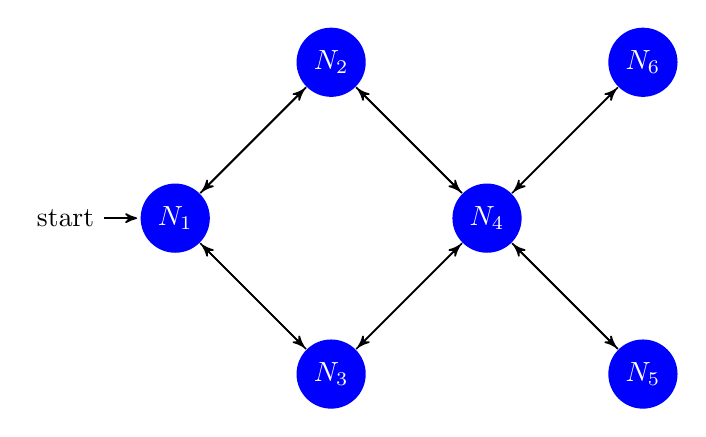
\begin{tikzpicture}[->,>=stealth',shorten >=1pt,auto,node distance=2.8cm,
                    semithick]
  \tikzstyle{every state}=[fill=blue,draw=none,text=white]

  \node[initial,state] (A)                    {$N_1$};
  \node[state]         (B) [above right of=A] {$N_2$};
  \node[state]         (D) [below right of=A] {$N_3$};
  \node[state]         (C) [below right of=B] {$N_4$};
  \node[state]         (E) [below right of=C] {$N_5$};
  \node[state]		   (F) [above right of=C] {$N_6$};

  \path (A) edge              node {} (B)
            edge              node {} (D)
        (B) edge              node {} (A)
        	edge			  node {} (C)
        (C) edge              node {} (B)
            edge 			  node {} (D)
            edge			  node {} (E)
            edge			  node {} (F)
        (D) edge 			  node {} (C)
            edge              node {} (A)
        (E) edge 			  node {} (C)
    	(F)	edge			  node {} (C);
\end{tikzpicture}
\\
%\[
%\begin{bmatrix}
%    x_{11}       & x_{12} & x_{13} & \dots & x_{1n} \\
%    x_{21}       & x_{22} & x_{23} & \dots & x_{2n} \\
%    \hdotsfor{5} \\
%    x_{d1}       & x_{d2} & x_{d3} & \dots & x_{dn}
%\end{bmatrix}
%=
%\begin{bmatrix}
%    x_{11} & x_{12} & x_{13} & \dots  & x_{1n} \\
%    x_{21} & x_{22} & x_{23} & \dots  & x_{2n} \\
%    \vdots & \vdots & \vdots & \ddots & \vdots \\
%    x_{d1} & x_{d2} & x_{d3} & \dots  & x_{dn}
%\end{bmatrix}
%\] 
The adjacent matrix becomes this matrix $[A]$: \\


$
\bordermatrix{
         & N_1		& N_2	& N_3	& N_4 	& N_5	&N_6     \cr
    N_1   & 0		& 1		& 1		& 0		& 0		& 0	     \cr
    N_2   & 1		& 0		& 0		& 1		& 0		& 0	     \cr
    N_3   & 1		& 0		& 0		& 1		& 0		& 0	     \cr
    N_4   & 0		& 1		& 1		& 0		& 1		& 1	     \cr
	N_5   & 0		& 0		& 0		& 1		& 0		& 0	     \cr
	N_6   & 0		& 0		& 0		& 1		& 0		& 0	     \cr
}$
\\

Matrix $A \times A = A^{2}$ becomes the matrix with the number of paths with 2 steps from $N_{i}$ to $N_{j}$: We denote this matrix as matrix \textit{[B]}\\


$
\bordermatrix{
         & N_1		& N_2	& N_3	& N_4 	& N_5	&N_6     \cr
    N_1   & 2		& 0		& 0		& 2		& 0		& 0	     \cr
    N_2   & 0		& 2		& 2		& 0		& 1		& 1	     \cr
    N_3   & 0		& 2		& 2		& 0		& 1		& 1	     \cr
    N_4   & 2		& 0		& 0		& 4		& 0		& 0	     \cr
	N_5   & 0		& 1		& 1		& 0		& 1		& 1	     \cr
	N_6   & 0		& 1		& 1		& 0		& 1		& 1	     \cr
}$
\\

Matrix $A^{2} \times A = A^{3}$ becomes the matrix with the number of paths with 3 steps from $N_{i}$ to $N_{j}$: We denote this matrix as matrix \textit{[C]}\\


$
\bordermatrix{
         & N_1		& N_2	& N_3	& N_4 	& N_5	&N_6     \cr
    N_1   & 0		& 4		& 4		& 0		& 2		& 2	     \cr
    N_2   & 4		& 0		& 0		& 6		& 0		& 0	     \cr
    N_3   & 4		& 0		& 0		& 6		& 0		& 0	     \cr
    N_4   & 0		& 6		& 6		& 0		& 4		& 4	     \cr
	N_5   & 2		& 0		& 0		& 4		& 0		& 0	     \cr
	N_6   & 2		& 0		& 0		& 4		& 0		& 0	     \cr
}$ 
\\

So for $A^{N}$ every $a_{ij}$ entry gives the number of paths with N steps from $N_{i}$ to $N_{j}$.\\

With this knowledge we can calculate in how many steps a node is infected. $A$ calculates which nodes are infected after 1 step, $A^{N}$ calculates which nodes are infected in N steps.. So if we want to know how many nodes are infected after 3 steps we have to add every matrix $(A + A^{2} + A^{3}) $ and see which entry is a non zero entry. 

What do we need for an algorithm
\begin{description}
\item Graph network $G = < V, E>$
\item Graph matrix $[A]$ which is $|V| \times |V| $
\item Attack vector $[X]$ which is $1 \times |V|$
\item cummulative matrix $[M]$ which is $|V| \times |V|$
\item state matrix $[T]$  which is $|V| \times |V|$
\item Reset vector $[R]$
\item duration \textit{d}
\item time \textit{n}
\item rate $\delta _{0}$ of defender and $\delta _{1}$ of attacker
\end{description}



Initialisation algorithm:


\begin{verbatim}
initialisatie
	d=0
	A=basismatrix
	M=A^{0}
	n=0
	\delta_{0}
	\delta_{1}
	X
	R
	controller = defender
	
	

	Algorithm
	n:= n + 1;
	Check who is in control? ( through modulo )
	if ( defender & controller=defender)
				d:= d + 1;
	
	if ( defender & controller=attacker )
				G = X \times R  (flippen ten voordele van defender)
				d = 0
				controller = defender
				
	if ( attacker & controller=defender )
				controller=attacker
				..
				
	if ( attacker & contoller=attacker )
				d:= d + 1
				M = M x A
				T = T + M
				G = X x T
				
		
\end{verbatim}

%\end{document}
\chapter{Intro to virus}
\label{cha:6}
%\documentclass[10pt]{article}\

%%%%%%%%%%%%%%%%%%%%%%%%%%%%%%%%%%%%%%%%%%%%%%%%%%%%%%%%%%
%%%%%			Introduction Chapter 6			%%%%%%
%%%%%												%%%%%%
%%%%%												%%%%%%
%%%%%%%%%%%%%%%%%%%%%%%%%%%%%%%%%%%%%%%%%%%%%%%%%%%%%%%%%%


\section{Introduction}
This section gives a formal definition of the FlipIt game with a virus propagation. First we derive a formula for a FlipIt game without a virus. After that we introduce a modification to this formula to achieve an adapted formula for a FlipIt game with a virus propagation. 
%In this section we are going to elaborate how we are going to model a Flipit game with multiple resources and a virus that propagates and infects the resources. We come up with a formula for the normal FlipIt (normal as in specific parameters and no normalising over the first interval) and then reform it to a FlipIt game with a virus. 

\subsection{FlipIt with a virus propagation}
In the previous section the FlipIt game is already been explained. In this section we will introduce a FlipIt game with a virus propagation. A FlipIt game with a virus propagation is a game where the attacker will drop a virus on one of the resources that is available. The virus will then spread itself to the neighbour resources. The attacker will only gain control over the whole network, in general the game, when it has infected all the resources. All the resources will not be infected immediately when the attacker has dropped its virus. It will take some time before the virus is spread and has infected everything. The time that it takes for the virus to infect every resource will be denoted as parameter \textit{d}. If we want to measure how long it takes for the virus to infect all resources, we have to calculate the shortest path to the farthest node. This can be measured by a method that we will explain in section []. With this parameter we can compose a formula to calculate the gain of a FlipIt game with a virus propagation.  \\ \todo{uitleggen waarom we een gewone flippit kunnen nemen met 1 resource}

The gain of a player is defined as the total amount of time that a player has owned the resource over the amount of time that has passed since the beginning of the game. If the attacker attacks with the virus it will cause a delay of length \textit{d}. This means that the gain of the player from the normal game has to be abstracted with a delay every time the attacker moves. This game, where the attacker drops a virus, cannot be modelled completely by a FlipIt game with a delay. This is because if the delay is bigger than the period of the attacker, the attacker will gain no control. If it would be with the delay caused by a phase bigger than zero the attacker would gain control after the defender flipt again. This is explained in figure \ref{fig:virusflip}. In the next section a formal definition .. \todo{verder uitleggen nog}

\begin{figure}[hbtp]
\caption{Difference in a FlipIt game between delay caused by a virus and a phase bigger than zero for the Attacker}
\centering
\includegraphics[scale=1]{Images/Flipvirus}
\label{fig:virusflip}
\end{figure}


\subsection{define formula}
The game FlipIt with a virus propagation is a two-player game with multiple resources. The multiple resources represent the nodes in a network. One of the players, the defender, will try to defend his network. The defender will do this by flipping all the nodes of the network in every move he plays. The attacker, the other player, will try to infect all the nodes in the network. The attacker will do this by flipping the node in the graph that can infect all the nodes in the shortest time possible. The attacker will gain the control over the network when all the resources are infected. So parameter \textit{d} will be the time of the shortest path from the start node to the furthest node. \\






Their is a definition given for the gain of a player \textit{i} by the writers of the paper FlipIt, but we want to add the property of a virus propagation to the game, hence parameter \textit{d}, so we are trying to find another formula that defines a game by counting the amount of time one of the players has control. \\

First a list of notations that will be used throughout the formal definition (see figure \ref{fig:notations} for a graphic representation of some of the notations):
\begin{description}
\item $\delta_{0}$: This is the period of the defender. This denotes the length of the interval between two consecutive moves of the defender. 
\item $\delta_{1}$: This is the period of the attacker. This denotes the length of the interval between two consecutive moves of the attacker.
\item \textit{$T_{0}$}: This denotes the phase of the attacker that was random and uniform chosen over the interval [0,$\delta_{0}$].
\item \textit{$T_{1}$}: This denotes the phase of the defender that was chosen uniformly at random in interval [0,$\delta_{0}$].
\item \textit{Unit of control}: Every continuous time step that one of the players has control over the resource is defined as a unit of control. 
\item \textit{n}: n is the n'th interval of the attacker, starting from interval 1.
\item $\Delta A$ : This is a function that denotes the length of a unit of control of the attacker in the n'th interval of the attacker.
\item \textit{lcm(a,b)}: The lcm of a and b is the least common multiple of a and b.
\item \textit{gcd(a,b)}: The gcd of a and b is the greatest common divider of a and b.
\end{description}
\begin{figure}[hbtp]
\caption{Defining unit of control}
\centering
\includegraphics[scale=1]{Images/FlipSpel.png}
\label{fig:notations}
\end{figure}

 
%\begin{equation}\label{first}
%n = \delta_{1} mod \delta_{0}
%\end{equation}
%
%\begin{equation}\label{first}
%\Delta A = [( \delta_{0} - n + 1 ) * \delta_{1}] mod \delta_{1}
%\end{equation}
%
%\begin{equation}\label{first}
%\sum_{i=0}^{\delta_{1}} \lbrace [( \delta_{0} - i + 1 ) * \delta_{1}] mod \delta_{1} \rbrace
%\end{equation}
%\todo{formule met i nakijken}


We \todo{We mag gebruikt worden in een wetenschappelijke tekst zolang de focus blijft op het werk en niet op de schrijver, FlipIt schrijvers gebruiken ook veel de we vorm} start by computing the gain of the attacker in a periodic game without phases. After that we introduce the phases. Next we compute the benefit of a player i in function of the gain. As last we adapt the computed formula for the gain and the benefit to formulate a new formula for a FlipIt game with a virus propagation. \todo{sectie over phases nog uitleggen}
\\
\subsubsection{Computing the benefit for an attacker of a normal FlipIt game}
\textbf{Case  1:} \\
For $delta_{1} > delta_{0}$ (The defender moves faster than the attacker.) \\

We consider a game in which both of the players start with a phase $T_{0}$ and phase $T_{1}$ equal to zero. Both players start their first move at $t=0$. As previously stated (in the formal definition of the game and the introduction of different notations used throughout the paper), the defender has control in the beginning of the game at $t=0$. If the two players move at the same time during the game, the moves cancel and no change of state happens. \\ \todo{eerder gedefinieerd dat elk spel begint op t=0}

To compute the gain formula for the attacker, we need to calculate the amount of time that the attacker has control over the game from the start of the game up to time t. This can be done by computing all the units of control of the defender up to time t \todo{formule is niet in staat om dat te doen als functie van t} and summarize it. \\
The formula that we are going to compute will not be in function of the time but in function of the intervals of the attacker. By doing this we always have a whole unit of control. If time is used the last unit of control can be shortened. Because the game goes on indefinitely and because it is easier to compute a formula in function of the intervals of the attacker, the gain formula will be in function of the intervals of the attacker. \todo{kan misschien beter uitgelegd worden}

For that reason we divide our time line of our FlipIt game into different intervals of size $delta_{1}$. Therefore every time the attacker moves we have the start of a new interval. Considering that the defender will move faster than the attacker, he or she will at least move one time during the interval of the attacker. Because the attacker only moves at the start of his or her interval we can say that the defender will always end as being in control of the resource. To calculate how long the unit of control of the attacker is in every interval, we only need to know how long the defender had control during that interval and substract it from the length of the interval of the attacker. 
\todo{blabla en dan hebben we de volgende formule}
This brings us to the next forumula to calculate the length of a unit of control in the n'th interval of the attacker. 
For every real number $delta_{1}$ and $delta_{0}$ and every n $\in$ of the natural numbers (including 0 in the set of natural numbers) :
\begin{equation}\label{first}
\Delta A = [( 1- n  ) \times \delta_{1}] mod \delta_{0}
\end{equation}
where n is the number of the n'th interval of the attacker where the length of the unit of control of the attacker is calculated.\\

%In this formula we multiply the number of unit of control that we want with the period of Attacker ( $\delta_{1}$). 
The 1 - n is when we count beginning from 1. If we start counting starting at 0 we leave the 1 and the formula becomes:
\begin{equation}\label{first}
\Delta A = [( - n  ) \times \delta_{1}] mod \delta_{0}
\end{equation}

%We know that each interval ends with the control for the defender. This means that we only need to know how long the defender had control during that interval and take the rest. The rest will be the amount of time the attacker has control in that interval. We take the rest by doing the $mod \delta_{0} $

For phases ..

This means that if we want to calculate the gain of the attacker we need to calculate the time the attacker has control over the total amount of time that has passed by.
For $\delta_{0}$ and $\delta_{1}$ $\in$ Rational numbers we can see that we have a cycle. A pattern that comes back over and over again. That is when the amount of time is a multiple of $\delta_{0}$ and $\delta_{1}$ or the largest common multiplier (lcm). At this point the Attacker and the Defender move at the same time what brings us back to the beginning.
So to calculate the gain of $\delta_{0}$ and $\delta_{1}$ $\in$ Rational numbers we need to calculate the amount of control units of the attacker that go into the length of time units equal to the lcm of  $\delta_{0}$ and $\delta_{1}$. After this calculation we divide it by the lcm of $\delta_{0} $ and $ \delta_{1}$, which is the total amount of time and the amount of time for one cycle.  This gives us the following formula:
\begin{equation}\label{first}
a = \dfrac{\delta_{0} }{lcm(\delta_{0},\delta_{1})} 
\end{equation}
\begin{equation}\label{first}
\dfrac{\sum_{i=0}^{a} \lbrace [( 1 - i ) \times \delta_{1}] mod \delta_{0} \rbrace \rbrace }{lcm(\delta_{0},\delta_{1})} 
\end{equation}

We can also define a formula without the greatest common divider. Every $\delta_{0}$ and $\delta_{1}$ have to be written in a fraction:
\begin{equation}\label{first}
\delta_{0}=\dfrac{a}{b} ~~~~and~~~~\delta_{1}=\dfrac{c}{d}
\end{equation}
If  $\delta_{0}$ or $\delta_{1}$ is a Geheel getal then b or d will be 1. The formula for the gain becomes different:\\

\todo{formule zoeken zonder lcm en gcd}


If $\delta_{0}$ and/or $\delta_{1}$ is an Irrational number:
An irrational number $ i \neq \dfrac{a}{b}$ with $b \in Z, a \in N$
Because we cannot write \textit{i} in a fraction, this means that we won't have a cycle. If we would have a cycle that means that we do have a number that divides \textit{i}. If we don't have a cycle it goes on forever. Meaning that it goes on to infinity. This also means that no number will be repeated two times. If it does that means that their is repetition, meaning again that their is a cycle. We can conclude that if we have no cycle and no number will be repeated twice, that it will enumerate every number between 0 and the biggest interval (which is $\delta_{0}$). \todo{interval definieren}
\textit{The reals are uncountable; that is: while both the set of all natural numbers and the set of all real numbers are infinite sets, there can be no one-to-one function from the real numbers to the natural numbers} [WikiPedia: real numbers] If they are uncountable that means that we cannot calculate the sum of all the numbers between 0 and the biggest interval. This is proved by the Cantor diagonalisation argument. Uncountable does not mean that we cannot order it. The Field of the real numbers is ordered. 

What we can do is take the limit, count as many control units of time of the attacker and divide it by the greatest amount of time. We can see that this eventually will result to the solution given by the writers of FlipIt. [r/2]. Example delta1 Pi and delta0 1. Grafiek voor maken.


\subsection{Formula with a virus propagation}
Now we can define how we can use the previous formula to calculate the benefit of the attacker with a virus propagation.
As mentioned before we have a parameter \textit{d} that defines the virus propagation. It will take an amount of time d before the attacker gains control over all the resources. We know how to calculate each unit of control of the attacker. If it takes d time before it can take control we have to subtract d form each unit of control. It can be that the unit of control is less than d. This means that we will have a negative number of time. In this case this means that the defender has flipped all the resources before the attacker good gain all the control. So if we want to calculate the benefit we can only take unit of control that are bigger than 0. So the formula becomes:

\begin{equation}\label{first}
\dfrac{\sum_{i=0}^{\delta_{0}} \lbrace [( 1 - i ) \times \delta_{1}] mod \delta_{0} - d \rbrace  > 0 \rbrace }{delta_{0} \times delta_{1}} 
\end{equation}

\subsection{Random phase}
For now we assumed that the first move of both players started at phase $t=0$. In the FlipIt game the first move is chosen uniformly over the interval [0,$\delta$]. We will call this first move the phase move and denote it by $T_{1}$ for the attacker and $T_{0}$ for the defender.
We will have to integrate these two phases into the formula.  
%\begin{equation}      
%\boxed{\eta \leq C(\delta(\eta) +\Lambda_M(0,\delta))}
%\end{equation}
%
%\begin{equation}\label{first}
%a=b+c
%\end{equation}
%
%\begin{subequations}\label{grp}
%\begin{align}
%a&=b+c\label{second}\\
%d&=e+f+g\label{third}\\
%h&=i+j\label{fourth}
%\end{align}
%\end{subequations}



%%% Local Variables: 
%%% mode: latex
%%% TeX-master: "thesis"
%%% End: 



\chapter{APT}
\label{cha:7}
%\documentclass[10pt]{article}\

%%%%%%%%%%%%%%%%%%%%%%%%%%%%%%%%%%%%%%%%%%%%%%%%%%%%%%%%%%
%%%%%			Introduction Chapter 7			%%%%%%
%%%%%												%%%%%%
%%%%%												%%%%%%
%%%%%%%%%%%%%%%%%%%%%%%%%%%%%%%%%%%%%%%%%%%%%%%%%%%%%%%%%%


\section{Advanced Persistent Threats}

A targeted attack follows most of the time a serie of stages to attack its victim. This pattern of stages is also know as the Kill Chain, first mentioned by .. []. An APT will not always follow exact each step of this chain but it will give a good guideline of how an APT works. 
\begin{enumerate}
\item \textbf{Reconnaissance}: During the first step of the Kill Chain an attacker will look for information to find an interesting victim. This information can be emailaddresses, IP addresses, conference information, anything that is available about the victim.
\item \textbf{Weaponization}: In the second stage the attacker will use an exploit and add a malicious playload to be send to the victim. 
\item \textbf{Delivery}: The attacker will deliver his malicious code to the victim through different kins of intrusion methods. This can include email, usb stick, cd's, web, applications or other means.
\item \textbf{Exploitation}:The attacker executes the exploit, which is only relevant if the attacker uses an exploit.
\item \textbf{Installation}: The malware will be installed on the asset. This is only relevant if the attacker uses malware as a part of the attack.
\item \textbf{Command and Control}: The attacker will set up a command and control channel for remote manipulation of the victim.
\item \textbf{Actions on Objectives}: With ''hands on keyboard'' access, intruders accomplish their original goal. 
\end{enumerate}
\todo{nog uitbreiden, toevoegen that attackers will stay unnoticed for as long as possible or leave unnoticed with sensitive information}

\includegraphics[scale=0.7]{Images/chainAPT} 
% ... en zo verder tot
\chapter{The Final Chapter}
\label{cha:n}


\section{chap}

%%% Local Variables: 
%%% mode: latex
%%% TeX-master: "thesis"
%%% End: 

\chapter{Conclusion}
\label{chapter5:conclusion}

This paper presents an adaptation to the basic FlipIt game by \citep{FlipIt} to model an attacker with a delay.  We list a set of extensions that might be interesting for further research.
\section{Further work}

\begin{description}
\item \textit{Nash equilibria}\\ This paper concluded with the best responds functions of the attacker and the defender. The next step would be to calculate the Nash equilibria. For these calculation multiple cases have to be examined. All the possible cases regarding $k_{A}, k_{D}$ and $d$. 
\item \textit{Analysing other renewal strategies} \\ By analysing other renewal strategies, it might be interesting to find out if the original result regarding periodic and renewal strategies of the basic FlipIt game still stands. This result was that periodic strategies strongly dominate the other renewal strategies if an opponent plays with a non-adaptive strategy. 
\item \textit{Delay for the defender}\\ This paper only assumed that the attacker had a delay. It could be interesting to have a defender with a delay. This situation could happen when it takes some time to make a patch a system or when a new exploit is found. 
\item \textit{Variable delay} \\This paper assumed that the propagation delay had a fixed value. This can be relaxed by giving the attacker a delay that can vary every flip. The delay is always negative for the attacker, so the attacker will always choose the lowest delay. But if the attacker always sends a new worm at every flip, it could be that the delays vary. So a variable delay would be more accurate to simulate a real world case. 
\item \textit{The defender flips a subset of nodes} \\ Our model assumes that if the defender flips, he flips the whole network. An option for the defender would be to flip a subset of nodes in the network. If the costs of the flipping are related to the amount of nodes that are flipped, this option might be interesting to look at. It could be that a certain subset of nodes is found that protects the whole network. The PageRank matrix explained in Chapter 5 can help with finding the right nodes. \\

\end{description}


\section{General results and conclusions}
Our FlipIt model with worm propagation delay showed us some interesting results. 
\begin{itemize}
\item When the defender plays faster than the delay, the attacker will either have a negative benefit or a benefit equal to zero if the flips do not cost anything. It is for the defender a target to be able to play at a rate smaller or equal to the delay.
\item If the defender can play with a cost equal to zero, the attacker will not play. The defender can play at any rate he wants, and the attacker is always disadvantaged by his delay.
\item From a certain value for the speed of the attacker, the defender will not play any more or will play at the same rate. The same for the attacker.
\end{itemize}

As of today APTs become more and more extraordinary pieces of malicious code. There are APTs known to survive military-grade disk wiping and reformatting, and even after the reformatting and reinstalling the operating system are able to send sensitive data (Equation group \citep{Equation}). This means that even if you know that an APT is on your network, the actual practical "flip" has to exist or known by the defender.  \\
The best way to secure a system is to find the weakest link. This is mostly the employee. To counter this problem, you have to raise the awareness of the risks.  Awareness is very important. Even if you have good security protection layers, spam filters, firewalls, a phishing mail opened by one of your employees or a USB stick is enough to infect a pc on the network and by that it can spread further. But a system can never be 100\% waterproof. If an infection has occurred and the defender knows a counter measure, the FlipIt game will help to prevent a system to be compromised. 
%%% Local Variables: 
%%% mode: latex
%%% TeX-master: "thesis"
%%% End: 


% Indien er bijlagen zijn:
\appendixpage*          % indien gewenst
\appendix
\chapter{The First Appendix}
\label{app:A}
\includepdf[pages=-]{paper.pdf}


%%% Local Variables: 
%%% mode: latex
%%% TeX-master: "thesis"
%%% End: 

% ... en zo verder tot
\chapter{The Last Appendix}
\label{app:n}
\includepdf[pages=-]{finaal.pdf}


%%% Local Variables: 
%%% mode: latex
%%% TeX-master: "thesis"
%%% End: 


\backmatter
% Na de bijlagen plaatst men nog de bibliografie.
% Je kan de  standaard "abbrv" bibliografiestijl vervangen door een andere.
\bibliographystyle{abbrv}
\bibliography{references}

\end{document}

%%% Local Variables: 
%%% mode: latex
%%% TeX-master: t
%%% End: 

